\section{Results}

In the previous section we defined a regime based trading strategy that uses an HMM as a times series forecasting model, which feeds into a model predictive control (MPC) framework to determine trading decisions. In this section results of the MPC strategy is evaluated and compared to a number of alternative portfolios. The analysis is divided between in-sample training and out-of-sample testing. The purpose of the in-sample training is to compute optimal values for hyperparameters of the forecast horizon and other hyperparameters in the MPC problem in \cref{eq: maximizing objective MPC}, while in the out-of-sample section, the MPC approach is evaluated using optimal parameters and compared to benchmarks. In the remainder of the section, we first present the data in- and out-of-sample, before describing the in-sample training after which out-of-sample results are presented.

\subsection{Data}

\textbf{Vi skal lige have en skarpere defintion af in-sample træning og så oos initialization og oos evaluation sets.}

The full dataset covers the period form February 1994 to February 2021. Though some indices go further back, the choice of time period is a trade-off between historical availability and the size of the asset universe, with the latter significantly shrinking before 1994. The in-sample data, shown in \cref{fig:MPC_data_is}, runs from February 1994 to November 2003, resulting in 2539 daily observations. It covers the S\&P 500, MSCI Emerging Markets, Barclays US Treasury, CSI Barc Index, Gold and Oil\footnote{
The 6 indices are \textbf{Insert formal name of all indices as indice 1, indice 2 etc.}.
}.
Three month treasury bills are used as a benchmark for the risk-free asset. In the initial months where only monthly data is available for the risk-free asset, daily prices are linearly interpolated with some gaussian noise. We note that the first 1700 observations are used for initialization after which training commences. As this is a rather large slice of the in-sample data implications of this is discussed in greater detail in the coming sections. Finally, we note that the assets considered in-sample is only a subset of the assets considered out-of-sample due to data limitations. \textbf{Consider implications of this on the optimal MPC hyperparameters.}

\begin{figure}[H]
    \centering
    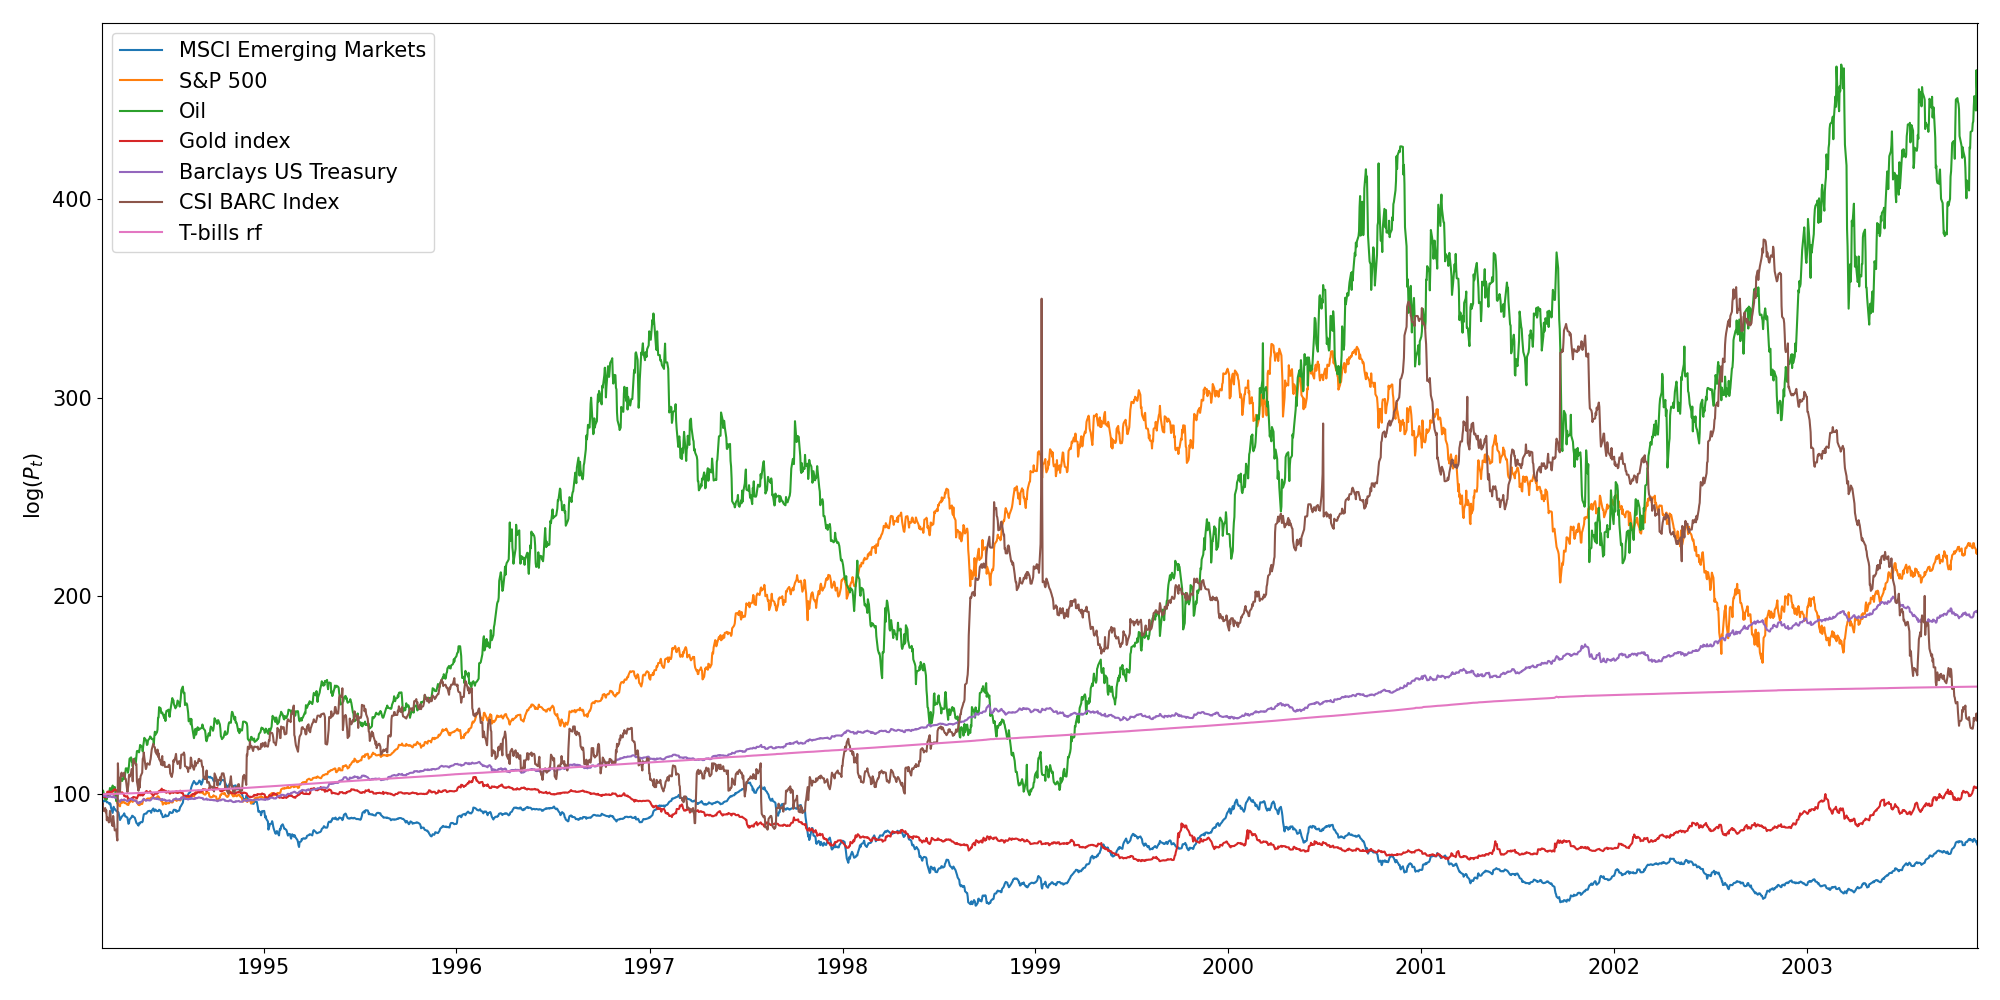
\includegraphics[width=1\textwidth]{analysis/portfolio_exercise/images/asset_vals_insample.png}
    \caption[Historical asset prices during the in-sample period]{Historical asset prices during the in-sample period.}
    \label{fig:MPC_data_is}
\end{figure}

The out-of-sample period runs from November 2003 to February 2021 resulting in 4495 daily observations. It is shown in \cref{fig:MPC_data_oos} It covers S\&P 500, MSCI Emerging Markets, Hedge Funds Global, Private Equity, European Public Real Estate, Gold, Oil, Barclays US Treasury and CSI Barc Index\footnote{
The 9 indices are \textbf{Insert formal name of all indices as indice 1, indice 2 etc.}.
}.
Again, the first years are used for initialization, meaning the the trading strategy is not implemented until September 2007, just before the financial crisis. This makes it an interesting period to study, as most assets had significant drawdowns during the crisis, and because it additionally includes the sovereign debt crisis in 2012 and the Covid-19 outbreak in 2020. As note by (\textbf{Insert REF}), asset correlations tend to increase during recessions, as can be seen in \cref{fig:MPC_data_oos}, meaning that many portfolios, such as an equally weighted or value weighted portfolio generally would suffer significant drawdowns in such periods. 

\begin{figure}[H]
    \centering
    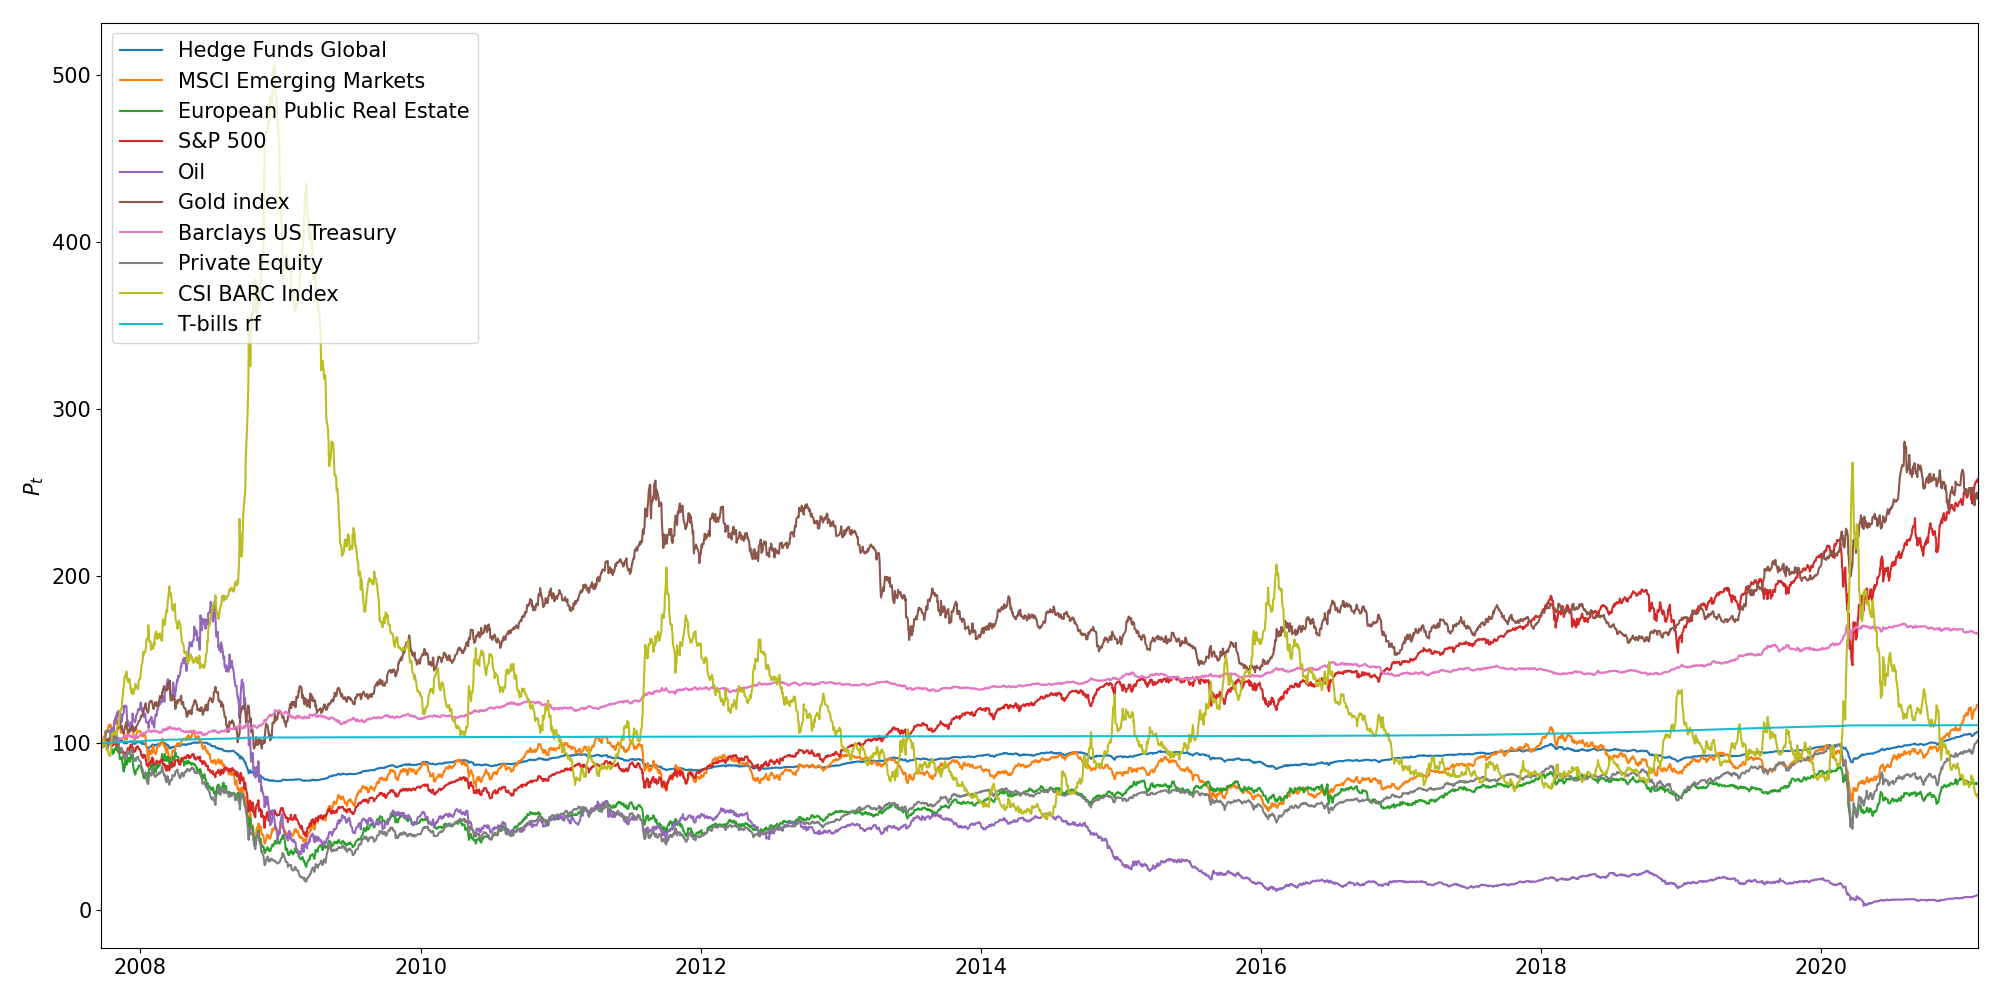
\includegraphics[width=1\textwidth]{analysis/portfolio_exercise/images/asset_vals_oos.png}
    \caption[Historical asset prices during the out-of-sample period]{Historical asset prices during the out-of-sample period. The dashed vertical line indicates the end of the initialization period and the beginning of the evaluation period. \textbf{Vis den fulde oos periode og forklar at de første 1700 observationer er brugt til initialization}}
    \label{fig:MPC_data_oos}
\end{figure}

Finally, \cref{tab:MPC_asset_performance} shows the annualized\footnote
{Daily returns are analyzed using
\begin{flalign*}
    \mu_{annual} &= (1+\mu_{daily})^{1/252}-1 \\
    \Sigma_{annual} &= {\Sigma}_{daily} * 252
\end{flalign*}
}
asset performance for the evaluation period 2007-2021. There is a clear difference in performance across the spectrum, and the fact that the sample period starts right before the GFC, i.e. at an all-time high, significantly worsens the results of most assets in the universe. This is clearly evident from negative sharpe ratios, as some of the assets still haven't recovered their pre-crisis prices and have performed worse than the risk-free asset over the evaluation period. Importantly, it should be noted that many of the assets have significantly better performances during subsets of the evaluation period, so conditional on being able to choose the right assets at the right time, a regime based strategy should be able to outperform benchmarks. Here it should be noted, that the chosen period is particularly interesting to study when the goal is to minimize portfolio drawdowns, as \cref{tab:MPC_asset_performance} generally indicates very high MDDs (Maximum Drawdown) and thus quite low calmar ratios\footnote{
Calmar ratio is defined as excess return divided by maximum drawdown.
},
it will be interesting to see whether MPC with drawdown control can mitigate this.

\begin{table}[H]
\small
\centering
\caption[Annualized
performance for each asset during the out-of-sample period]{Annualized
performance for each asset during the out-of-sample evaluation period 2007-2021. All measures are in excess of the risk-free rate.}
\begin{tabular}{lrrrrrrr}
\toprule
{} &  return &     std &  excess\_return &  excess\_std &  sharpe &  max\_drawdown &  calmar\_ratio \\
\midrule
MSCI World            &  0.0338 &  0.1638 &         0.0180 &      0.1641 &  0.1094 &        0.5907 &        0.0304 \\
MSCI Emerging Markets &  0.0591 &  0.1869 &         0.0429 &      0.1872 &  0.2291 &        0.6606 &        0.0649 \\
S\&P 500               &  0.0459 &  0.1923 &         0.0299 &      0.1925 &  0.1553 &        0.5678 &        0.0527 \\
Oil                   & -0.0800 &  0.3928 &        -0.0941 &      0.3929 & -0.2395 &        0.9852 &       -0.0955 \\
Gold index            &  0.0929 &  0.1681 &         0.0762 &      0.1680 &  0.4537 &        0.4462 &        0.1708 \\
Barclays US Treasury  &  0.0427 &  0.0443 &         0.0268 &      0.0440 &  0.6099 &        0.0717 &        0.3742 \\
CSI BARC Index        & -0.0428 &  0.3155 &        -0.0573 &      0.3153 & -0.1818 &        0.8925 &       -0.0642 \\
port\_val              &  0.0530 &  0.0967 &         0.0370 &      0.0965 &  0.3828 &        0.2671 &        0.1384 \\
\bottomrule
\end{tabular}

\label{tab:MPC_asset_performance}
\end{table}

\subsection{In-sample training}

In-sample training is performed by evaluating three distinct objectives. Concretely, we are interested in maximizing the sharpe ratio, maximizing the calmar ratio and minimizing portfolio turnover. That is, just as in a regular Markowitz mean-variance setting, high excess returns and low standard deviations are preferred, though with the added objective that, for a given return and standard deviation, a lower drawdown over the period is preferred. Minimizing annual turnover is imposed as a means of regularizing the amount of trades ocurring, and thus minimizing actual trading costs incurred. Training is carried out for a long-only portfolio with $\gamma_0=5$ because that results in excess risk similar to the 1/n portfolios\footnote
{Refer to the out-of-sample section to see a range of $\gamma_0$.
}. Furthermore, $D_{max}$ is set to 0.15 - the choice of this parameter is arbitrary as it is up to the individual portfolio manager to determine how much drawdown she will allow in practice. Finally, one-way transaction costs are assumed to be 10 basis points, while there are zero costs associated with trading the risk-free asset. This is a realistic assumption for institutional investors (Nystrup et al, 2017).

The training is quite challenging because many of the hyperparameters are mutually dependent, meaning we have to test all combinations within a specified grid. One of the advantages of the MPC approach, as outlined in \cref{algo:MPC}, is the complete separability between forecasting expected conditional asset parameters $\hat\mu_{t+H}$ \& $\hat\Sigma_{t+H}$ and solving for the optimal sequence of trades in \cref{eq: maximizing objective MPC}. Therefore, to reduce training time, the set of predicted means and covariances for each asset can first be computed for the set of hyperparameters relating to the forecast model, i.e. length of forecast horizon H, size of shrinkage factors $\upsilon$ etc. This can then stored into memory after which tuning the MPC hyperparameters can be performed.

\subsubsection*{Forecasting model}

\subsubsection*{MPC parameters}

\paragraph{\textbf{Planning horizon.}} Planning horizons of $H=1,10,15,25$ are tried. 15 days appear to be optimal as 1 and 10 days are too few and 25 is too many.

\paragraph{\textbf{Transaction costs.}} We test transaction costs $(\kappa_1)_{1:n}=0.0005, 0.001, 0.004, 0.008, 0.012, 0.015$. As mentioned previously, there is no transaction costs incurred for the risk-free asset. $(\kappa_1)_{1:n}=0.0010$ appear to maximize the objectives. For this parameters, we find similar results as those of Nystrup et al. (2017), with the $\ell_1$ term $\kappa_1^T|w_t-w_{t-1}|$ being quite effective at reducing turnover, whilst the $\ell_2$ term $\kappa_2^T(w_t-w_{t-1})^2$ does not appear to provide additional value as it penalizes large one-day trades by splitting them into multiple days.

\paragraph{\textbf{Holding costs.}} Holding costs $(\rho_2)_{1:n+1}=0, 0.0001, 0.0005, 0.001, 0.002$ are tested, with $(\rho_2)_{1:n+1}=0.0020$ being optimal. Contrary to transaction costs, we impose a cost for holding the risk-free asset as it decreases the general allocation to cash. \textbf{Consider increasing the holding cost of rf.} For the holding costs the $\ell_2$ term $\rho_2^Tw_t^2$ is effective at increasing portfolio diversification as allocations to an asset is quadratically penalized. The $\ell_1$ term $\rho_1^T|w_t|$ does not change much. Having a holding cost complements a maximum holding constraint.

\paragraph{\textbf{Maximum holding constraint.}} Maximum holding constraints $(w_t)_{1:n}^{max}=0.2,0.3,0.4,0.5,$ is tested. 0.2 appear most effective. \textbf{0.5 might actually be better, need to run algo again.}


\subsection{Out-of-sample results}

In this section the model specified in the section above is run on the out-of-sample data and evaluated on the evaluation set. Initially, portfolio allocations and price developments are shown for a variety of borrowing constraints and for different values of $D_{max}$, using $\gamma_0=5$. Then, the analysis is expanded to also include a grid of risk aversion parameters $\gamma_0$, in which a variety of efficient frontiers and indifference curves are analyzed. Again, a fee of 10 basis points per one-way transaction is assumed, not including the risk-less asset, and the fee for shorting assets is assumed equal to the risk-free rate. There are assumed no price-impacts upon trading and no holding costs.

\subsubsection*{Allocations}

\textbf{Hvis resultater er ens så noter at resultater er de samme mellem mle og jump.}


\begin{figure}[H]
    \centering
    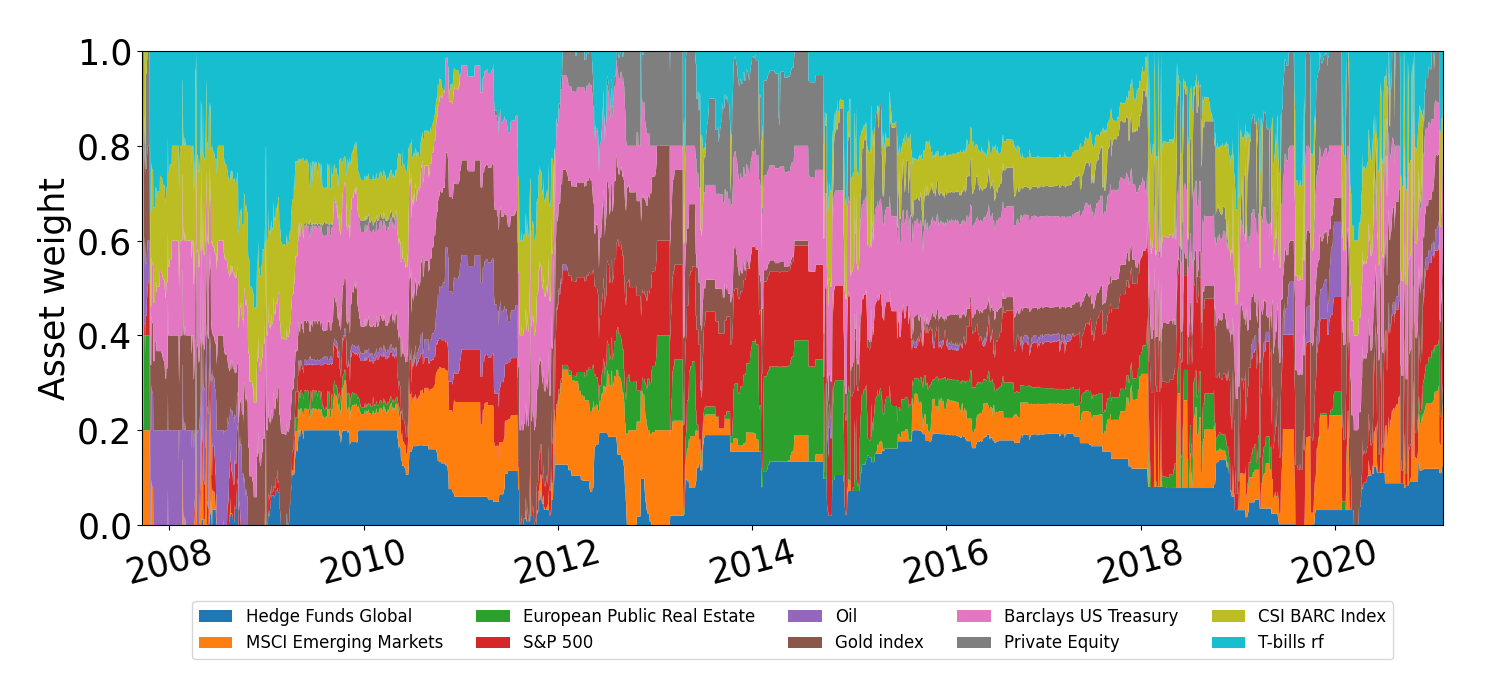
\includegraphics[width=1\textwidth]{analysis/portfolio_exercise/images/mle/weights_lo.png}
    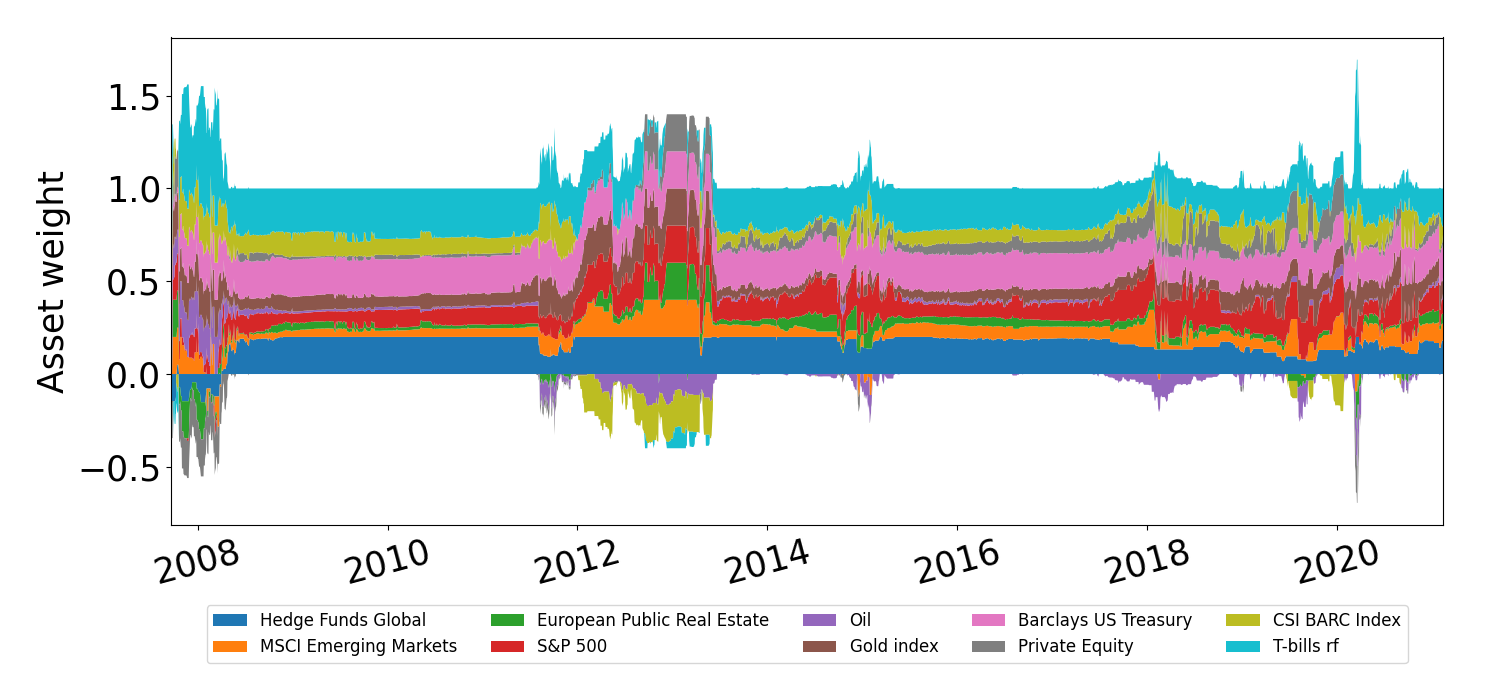
\includegraphics[width=1\textwidth]{analysis/portfolio_exercise/images/mle/weights_ls.png}
    \caption[Asset weights over time for a long-only portfolio]{Asset weights over time for a long-only portfolio.}
    \label{fig:MPC_port_weights_lo}
\end{figure}

\subsubsection*{Performance comparison}

\textbf{$D_{max}$ indikerer den maksimale drawdown tolerance. Hvis en portefølje når $D_{max}$, går risikoaversionen $\gamma$ mod uendelig. Alle plots er efter transaction costs på 10 basispoint per one-way transaktion.}

\begin{table}[H]
\centering
\caption[]{}
\begin{tabular}{lrrrrr}
\toprule
{} &  Excess Return &  Excess Std &    Sharpe &  Max drawdown &  Calmar ratio \\
\midrule
\$LO\_\{D\_\{max\}=0.15\}\$ &       0.033400 &    0.071954 &  0.464191 &      0.157512 &      0.212049 \\
LO                  &       0.033910 &    0.080413 &  0.421703 &      0.212418 &      0.159640 \\
\$LS\_\{D\_\{max\}=0.15\}\$ &       0.042353 &    0.103096 &  0.410808 &      0.177290 &      0.238889 \\
LS                  &       0.054931 &    0.144995 &  0.378849 &      0.366552 &      0.149859 \\
FM                  &       0.025461 &    0.032719 &  0.778164 &      0.119720 &      0.212668 \\
1/n                 &       0.017934 &    0.087748 &  0.204385 &      0.350445 &      0.051176 \\
\bottomrule
\end{tabular}

\label{tab:mpc_performance}
\end{table}

\begin{figure}[H]
    \centering
    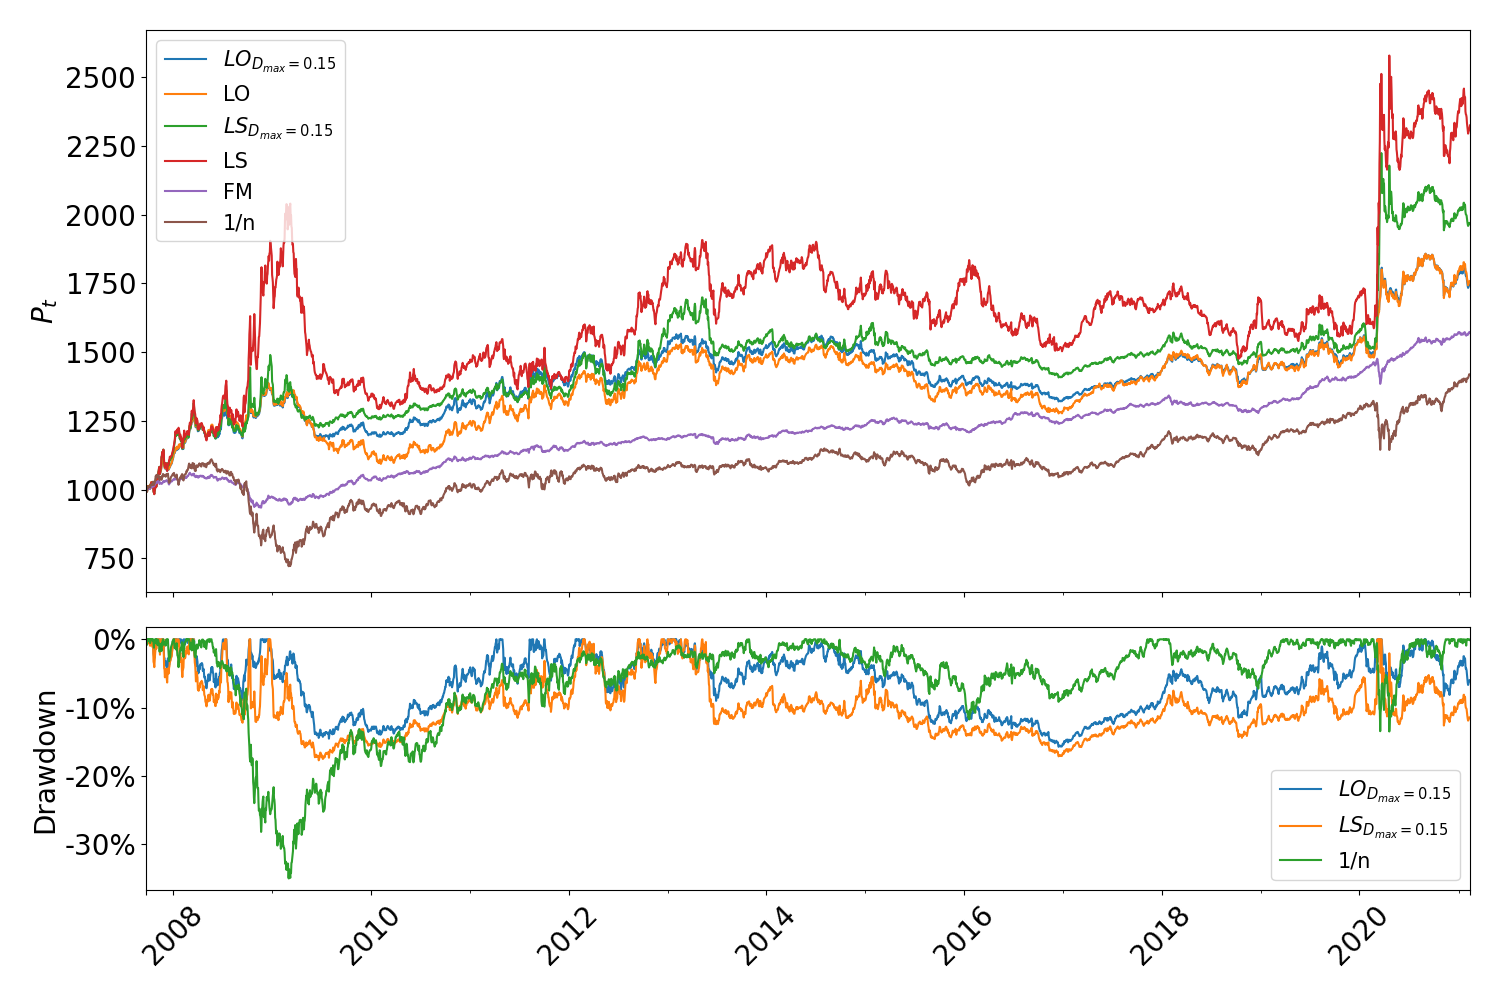
\includegraphics[width=1\textwidth]{analysis/portfolio_exercise/images/comparison_perf.png}
    \caption[Comparison of MPC investment strategies for various values of $D_{max}$]{Comparison of MPC investment strategies for various values of $D_{max}$.}
    \label{fig:MPC_port_vals_lo}
\end{figure}

\subsubsection*{Efficient frontiers}

\begin{figure}[H]
    \centering
    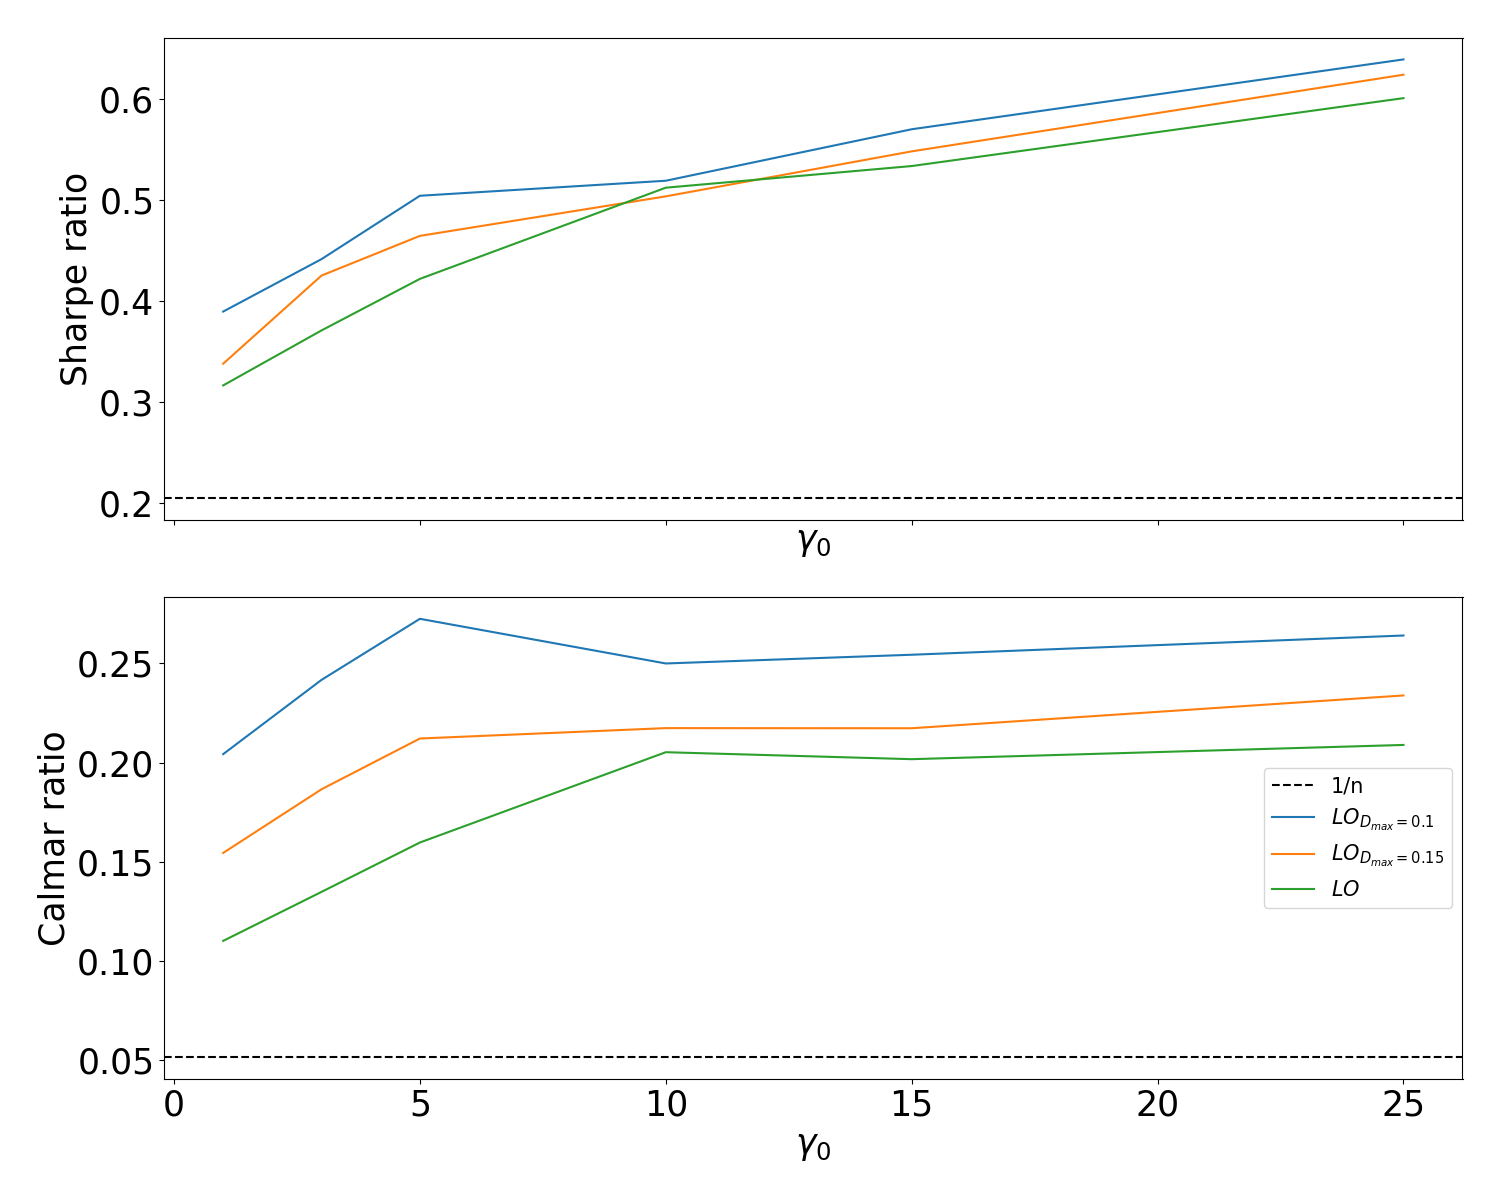
\includegraphics[width=1\textwidth]{analysis/portfolio_exercise/images/mle/sharpe_frontier_lo.png}
    \caption[Sharpe and Calmar ratio as function of $\gamma_0$ various values of $D_{max}$]{Sharpe and Calmar ratio as function of $\gamma_0$ various values of $D_{max}$.}
    \label{fig:MPC_sharpe_frontier_lo}
\end{figure}

\begin{figure}[H]
    \centering
    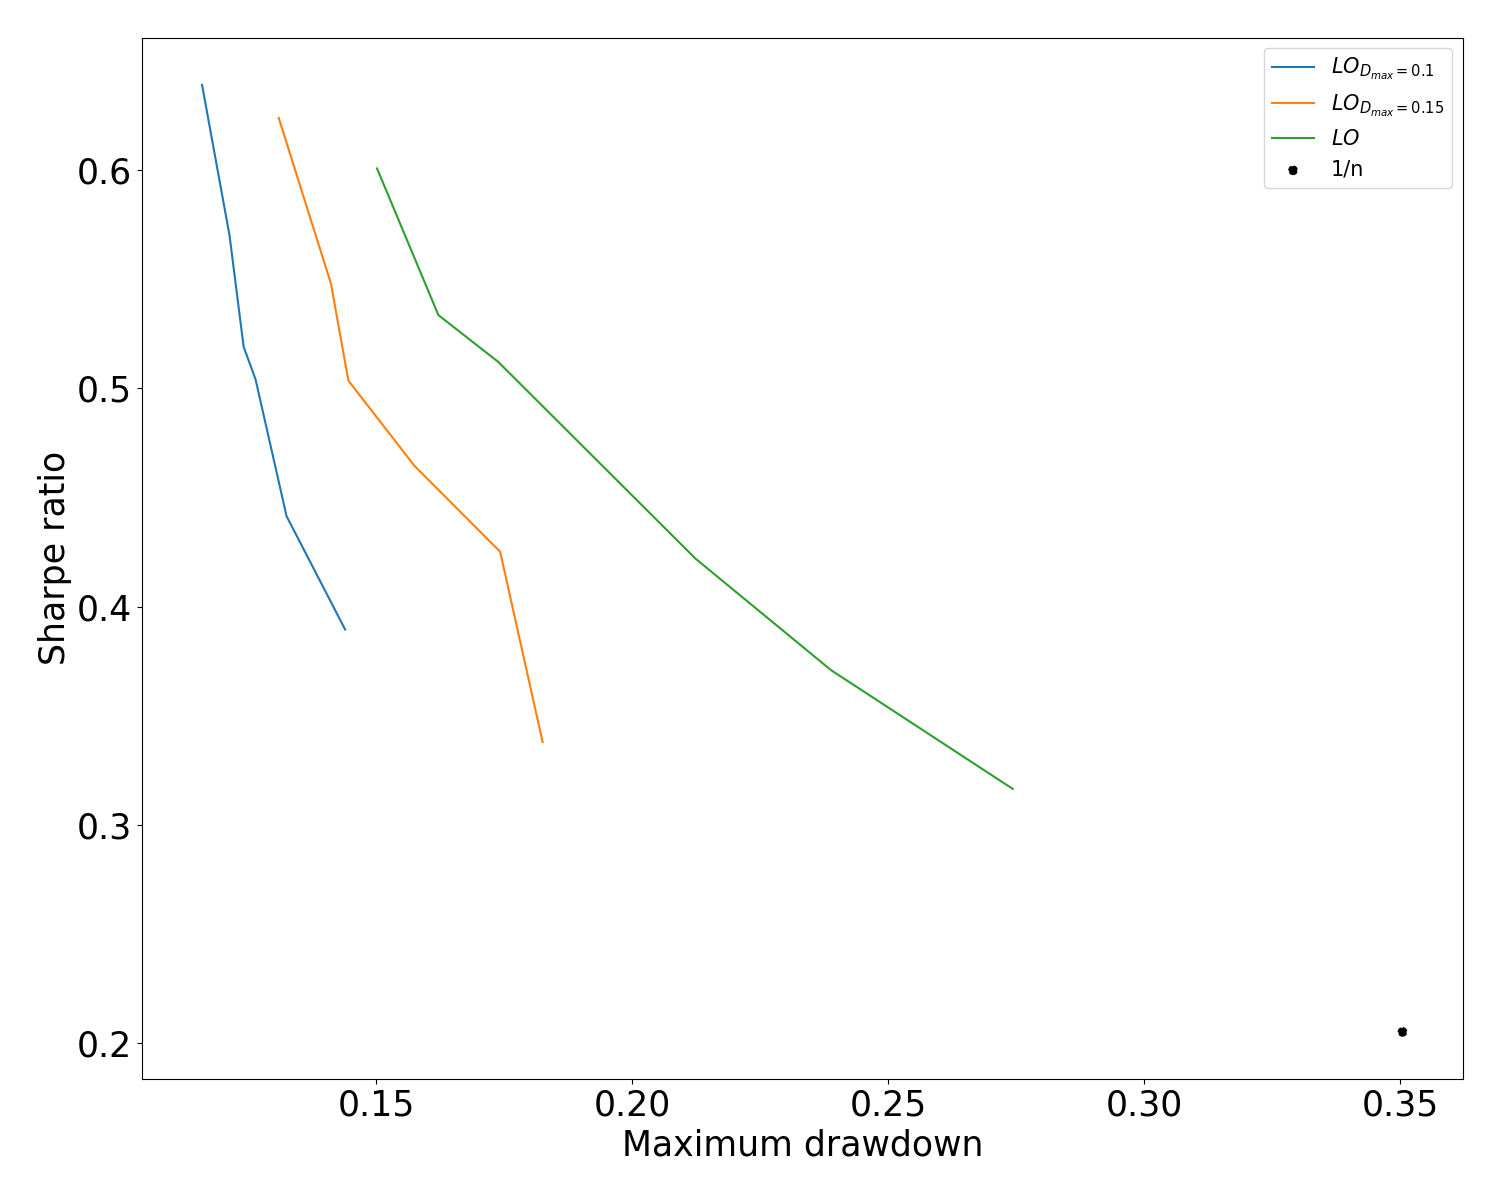
\includegraphics[width=1\textwidth]{analysis/portfolio_exercise/images/mle/sharpe_mdd_lo.png}
    \caption[Sharpe as function of MDD for various values of $D_{max}$]{Sharpe as function of MDD for various values of $D_{max}$. The points from right to left correspond to $\gamma_0=1,3,5,10,15,25$}
    \label{fig:MPC_sharpe_mdd_lo}
\end{figure}

\subsubsection{Comparison}